  \documentclass[11pt,a4paper]{article}

  \usepackage[margin=1in]{geometry}
  \usepackage{amsmath}
  \usepackage{pgfplots}
  \pgfplotsset{compat=1.18}
  \usepackage{booktabs}
  \usepackage{microtype}
  \usepackage{parskip}
  \usepackage{enumitem}

  \title{\textbf{Assignment 3}\\[0.3em]
  \large COL380}
  \author{Popat Nihal Alkesh (2023CS10058)}
  \date{April 2026}

  \begin{document}
  \maketitle

  % =============================================================================
  \section{Parallelisation Strategy}

  The parallel solver uses a \textbf{dynamic task-pool} model over MPI One-Sided
  (RMA) communication, operating in three phases.

  \textbf{Phase 1 --- Task generation.}
  Rank~0 expands the B\&B tree to a shallow depth (1 or 2 levels, chosen so at
  least $4\times\text{nprocs}$ tasks are created) to produce a pool of independent
  subproblems.  The best profit found during generation is broadcast to all ranks
  as an initial pruning bound, then the serialised task list is broadcast via
  \texttt{MPI\_Bcast}.

  \textbf{Phase 2 --- Dynamic scheduling with RMA atomic counter.}
  An MPI window on rank~0 stores two integers: a task counter and the global
  $P_{\max}$.  Every rank atomically claims the next task with
  \texttt{MPI\_Fetch\_and\_op} (fetch-and-increment), solves it sequentially using
  the full B\&B with both bounds, and loops back for another.  There is no manager
  rank and no message-passing overhead per task.

  Every 500 B\&B nodes each rank pushes its local best to the global $P_{\max}$
  using \texttt{MPI\_Fetch\_and\_op} with \texttt{MPI\_MAX}.  This propagates
  tight pruning bounds to all ranks without barriers, enabling collaborative
  pruning across the search space.

  When fewer than $2\times\text{nprocs}$ tasks remain unclaimed, a split flag is
  raised and subsequent recursive calls donate unexplored sub-trees to a local
  spare buffer rather than exploring them.  At round end, spare tasks are gathered
  via \texttt{MPI\_Allgatherv} and form the next round's task pool, preventing
  idle ranks late in each round.

  \textbf{Phase 3 --- Result collection.}
  \texttt{MPI\_Allreduce} with \texttt{MPI\_MAXLOC} finds the rank with the best
  profit; that rank broadcasts its clique and rank~0 writes the output.

  % =============================================================================
  \section{Sequential Optimisations}

  Beyond parallelisation, several optimisations were applied to the sequential
  B\&B kernel itself.

  \textbf{Sorted candidate ordering.}
  The initial candidate set is sorted once by decreasing $p(v)/c(v)$ ratio and
  this order is preserved throughout the recursion: \texttt{C\_next} is always
  constructed as a subsequence of the parent's candidate list, so no re-sorting
  is ever needed.  This ordering simultaneously satisfies the greedy-first
  requirement of the fractional knapsack bound and front-loads high-value
  vertices so profitable cliques are found early, tightening $P_{\max}$ quickly
  and improving pruning from the very first branch.

  \textbf{Reusable coloring buffers.}
  The greedy coloring routine reuses two global structures across every recursive
  call: \texttt{color\_classes} (the list of color class vectors) and
  \texttt{color\_buf} (the sorted scratch array).  Only the classes used in the
  previous call are cleared at the start of the next call; unused trailing
  entries are left untouched.  This avoids repeated heap allocation and
  deallocation that would otherwise dominate in deep recursions.

  \textbf{Adjacency matrix as \texttt{uint8\_t}.}
  The adjacency matrix is stored as a flat $N \times N$ array of single bytes
  rather than booleans or bitsets.  Byte-sized elements avoid bit-unpacking
  overhead and fit well into cache lines during the inner adjacency checks of
  the coloring loop.

  \textbf{Pre-filtering by budget.}
  Vertices whose cost already exceeds $B$ are excluded from the candidate set
  before the search begins, reducing the search space without any B\&B overhead.

  \textbf{Candidate reservation.}
  \texttt{C\_next} is reserved to the size of the parent candidate list before
  being filled, avoiding incremental reallocations during the inner adjacency
  scan.

  % =============================================================================
  \section{Performance Results}

  All experiments used the provided test graph compiled with
  \texttt{mpic++ -O3 -std=c++17} and run via \texttt{mpirun -np N ./main\_new}.
  Execution time is the wall-clock \texttt{real} time reported by \texttt{time}.

  \begin{table}[h]
  \centering
  \caption{Execution time, speedup, and parallel efficiency vs.\ number of processes.}
  \label{tab:timing}
  \begin{tabular}{rrrr}
    \toprule
    \textbf{Processes} & \textbf{Time (s)} & \textbf{Speedup} & \textbf{Efficiency} \\
    \midrule
    1  & 8.076 & 1.00 & 1.000 \\
    2  & 4.184 & 1.93 & 0.965 \\
    4  & 2.304 & 3.51 & 0.877 \\
    8  & 1.428 & 5.66 & 0.707 \\
    12  & 1.175 & 6.87 & 0.573 \\
    16  & 1.103 & 7.32 & 0.458 \\
    \bottomrule
  \end{tabular}
  \end{table}

  \begin{figure}[h]
  \centering
  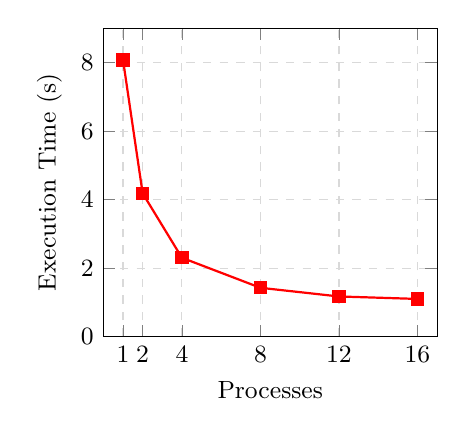
\begin{tikzpicture}
  \begin{axis}[
    width=0.48\textwidth, height=5.5cm,
    xlabel={Processes}, ylabel={Execution Time (s)},
    xmin=0, xmax=17, ymin=0, ymax=9,
    xtick={1,2,4,8,12,16},
    grid=major, grid style={dashed,gray!30},
    tick label style={font=\small}, label style={font=\small},
  ]
  \addplot[solid, thick, red, mark=square*, mark size=2pt]
    coordinates {(1,8.076)(2,4.184)(4,2.304)(8,1.428)(12,1.175)(16,1.103)};
  \end{axis}
  \end{tikzpicture}
  \hfill
  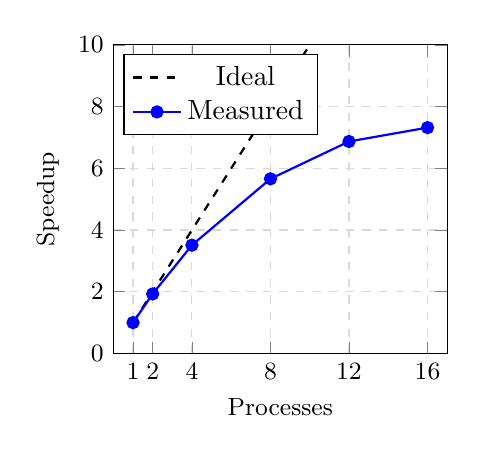
\begin{tikzpicture}
  \begin{axis}[
    width=0.48\textwidth, height=5.5cm,
    xlabel={Processes}, ylabel={Speedup},
    xmin=0, xmax=17, ymin=0, ymax=10,
    xtick={1,2,4,8,12,16},
    ytick={0,2,4,6,8,10},
    grid=major, grid style={dashed,gray!30},
    legend pos=north west,
    tick label style={font=\small}, label style={font=\small},
  ]
  \addplot[dashed, thick, black, domain=1:16, samples=50] {x};
  \addlegendentry{Ideal}
  \addplot[solid, thick, blue, mark=*, mark size=2pt]
    coordinates {(1,1.00)(2,1.93)(4,3.51)(8,5.66)(12,6.87)(16,7.32)};
  \addlegendentry{Measured}
  \end{axis}
  \end{tikzpicture}
  \caption{Execution time (left) and speedup vs.\ ideal (right) on the provided test graph.}
  \label{fig:perf}
  \end{figure}

  % =============================================================================
  \section{Discussion}

  Scaling is strong up to 8 processes (efficiency 0.707, speedup 5.66$\times$)
  and tapers off beyond that, reaching 7.32$\times$ at 16 processes
  (efficiency 0.458).  The diminishing returns past 8 processes are expected:
  the test graph's B\&B search tree has a finite amount of parallelism, and once
  enough ranks are active to exhaust the task pool quickly, the per-round
  \texttt{MPI\_Allgatherv} and \texttt{Allreduce} overheads become relatively
  more significant.  The pool-low splitting mechanism mitigates late-round
  idling but cannot fully recover the lost efficiency when individual tasks
  become very short.  Collaborative $P_{\max}$ synchronisation likely provides
  a speedup bonus by propagating tight bounds early, which is why the measured
  speedup is close to linear for small process counts despite the overhead of
  task generation and broadcasting.

  \end{document}
